\subsection{Cel ćwiczenia}
\quad To ćwiczenie ma na celu zapoznanie się z metodami generacji 
losowych punktów oraz badanie metod klasyfikacji położenia punktów na płaszczyźnie 
względem prostej. 
\subsection{Położenie punktu względem prostej}

\begin{wrapfigure}{r}{0.5\textwidth}

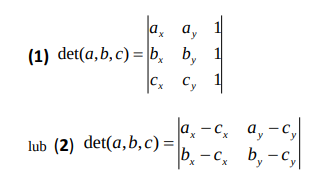
\includegraphics[width=7cm,scale=0.5]{./wyznaczniki.png}
\end{wrapfigure}

\quad Położenie punktu względem prostej będziemy wyznaczać obliczjąc
dane wyznaczniki. Wyznaczniki pozwalają określić położenie
punktu c względem prostej która jest wyznaczona przez punkty a i b.
Jeżeli wyznacznik jest większy od 0 to punkt znajduje się z lewej strony prostej, jeżeli jest mniejszy
od 0  to
punkt znajduje się po prawej stronie prostej, a jeżeli wartość wyznacznika
jest równa 0 (lub jej wartość bezwzględna $< \varepsilon$) to punkt leży na prostej.

\quad Pomimo, że
powyższe wyznaczniki są sobie równoważne to na skutek
niedoskonałości reprezentacji liczb rzeczywistych w komputerze wyniki
mogą się różnić w zależności od użytego wyznacznika.